\chapter{Probabilistic Principal Component Analysis}
\label{ch:ppca}

\section{From Discrete to Continuous Latent Variables}
So far we have studied probabilistic models with discrete latent variables, that is $z\in\{1,\ldots,K\}$. In particular we have discussed the Gaussian mixture model and the hidden Markov model, depicted in Figure~\ref{fig:gmm-hmm}.
\begin{figure}[H]
 \centering
 \begin{tikzpicture}[->]
    \node[latent] (z) {$z$};
    \node[obs,below=of z] (x) {$\bs{x}$};
    \edge{z} {x};
\end{tikzpicture}\hspace{2cm}
\begin{tikzpicture}[->]
    \node[latent] (zm) {$z_{t-1}$};
    \node[latent,right=of zm] (z) {$z_t$};
    \node[latent,right=of z] (zp) {$z_{t+1}$};
    \node[obs,below=of zm] (xm) {$\bs{x}_{t-1}$};
    \node[obs,right=of xm] (x) {$\bs{x}_t$};
    \node[obs,right=of x] (xp) {$\bs{x}_{t+1}$};
    \edge{zm} {z};
    \edge{z} {zp};
    \edge{zm} {xm};
    \edge{z} {x};
    \edge{zp} {xp};
\end{tikzpicture}
 \caption{Graphical representation of a GMM (left) and an HMM (right). \label{fig:gmm-hmm}}
\end{figure}

In the following courses we will discuss models with continuous $z$. This means that $\bs{z}\in\mathbb{R}$. The continuous equivalent of GMM is called probabilistic principal component analysis (PPCA), and the one corresponding to HMM is called Linear Dynamical System (LDS) and will be discussed in Chapter~\ref{ch:lds}.

\section{The PPCA Model}
The PPCA model uses some of the concepts and intuitions around the multivariate Gaussian distribution discussed in Chapter~\ref{ch:intro}. From a graphical perspective it is the same as GMM (left of Figure~\ref{fig:gmm-hmm}), but the nature of the random variables and their interdependencies change. \vspace{3mm}

\remark{ppca-model}{The PPCA model is characterised by:
\begin{itemize}
 \item Two continuous variables, one hidden one observed. Traditionally, $\bs{z}\in\mathbb{R}^{d_{\textsc{z}}}$ and $\bs{x}\in\mathbb{R}^{d_{\textsc{x}}}$ denote the hidden and observed dimensions, and $d_{\textsc{z}} \ll d_{\textsc{x}}$.
 \item The prior on the latent variable is a standard Gaussian:
 \begin{equation}
  p(\bs{z}) = \mathcal{N}(\bs{z};\bs{0},\bs{I}).
 \end{equation}
 \item The conditional likelihood is a multivariate Gaussian:
 \begin{equation}
  p(\bs{x}|\bs{z}) = \mathcal{N}(\bs{x};\bs{A}\bs{z}+\bs{b},\nu\bs{I}).
 \end{equation}
\end{itemize}}\vspace{3mm}

\exercise{ppca-free-param}{What is the number of free parameters of the PPCA model?}\vspace{3mm}

Alternatively, one can write $\bs{x}=\bs{A}\bs{z}+\bs{b}+\bs{\epsilon}$ with $\bs{\epsilon}\sim\mathcal{N}(\bs{\epsilon};\bs{0},\nu\bs{I})$, being $\bs{\epsilon}$ and $\bs{z}$ independent. An example of the generative process of PPCA can be found in Figure~\ref{fig:ppca-gen}.

\begin{figure}[H]
\centering\hfill
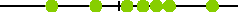
\includegraphics[width=0.22\textwidth]{fig/ppca_generation_1.pdf}\hfill
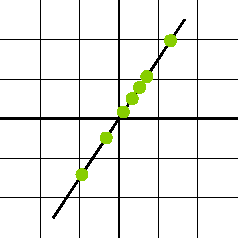
\includegraphics[width=0.22\textwidth]{fig/ppca_generation_2.pdf}\hfill
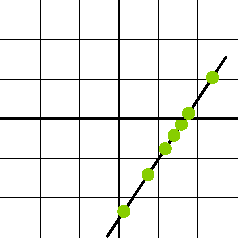
\includegraphics[width=0.22\textwidth]{fig/ppca_generation_3.pdf}\hfill
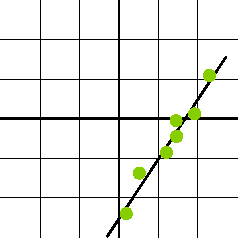
\includegraphics[width=0.22\textwidth]{fig/ppca_generation_4.pdf}\hfill
\caption{Example of the generative process of PPCA. From left to right. We first generate the low-dimensional latent variable $\bs{z}$, which gets multiplied by the linear operator $\bs{A}$, and added the bias $\bs{b}$, before adding the high-dimensional noise $\bs{\epsilon}$, to obtain the observations $\bs{x}$.\label{fig:ppca-gen}}
\end{figure}

\exercise{ppca-marginal}{Prove that, given the PPCA model, the marginal of $\bs{x}$ has mean vector $\bs{b}$ and covariance matrix $\bs{A}\bs{A}^\top+\nu\bs{I}$.}\vspace{3mm}

\exercise{ppca-marginal-2}{Prove that the shape of the marginal distribution $p(\bs{x})$ corresponds to the one of a multivariate Gaussian. To do so, first prove that the joint distribution in $\bs{x}$ and $\bs{z}$ can be expressed as:
\begin{equation}
 p(\bs{x},\bs{z})\stackrel{\bs{x},\bs{z}}{\propto} \exp\left(-\frac{1}{2}\left[ \frac{\|\bs{x}-\bs{b}\|^2}{\nu}-\bs{m}^\top\bs{\Omega}^{-1}\bs{m}\right]\right)\mathcal{N}(\bs{z};\bs{m},\bs{\Omega}),
\end{equation}
with
\begin{equation}
 \bs{\Omega} = \left(\frac{\bs{A}^\top\bs{A}}{\nu}+\bs{I}\right)^{-1} \qquad \bs{m}=\bs{\Omega}\left(\frac{\bs{A}^\top(\bs{x}-\bs{b})}{\nu}\right) .
\end{equation}
}\vspace{3mm}

While it is clear from the previous equation that the mean of the marginal distribution is $\bs{b}$, understanding that the corresponding covariance matrix is what was found in Exercise~\ref{ex:ppca-marginal} is not trvial. You might use the \textbf{Woodbury matrix inversion lemma}:\vspace{3mm}

\remark{woodbury}{For matrices $\bs{D}\in\mathbb{R}^{n\times n}$, $\bs{U}\in\mathbb{R}^{n\times m}$, $\bs{C}\in\mathbb{R}^{m\times m}$ and $\bs{V}\in\mathbb{R}^{m\times n}$, the following identity holds:
\begin{equation}
 (\bs{D} + \bs{U}\bs{C}\bs{V})^{-1} = \bs{D}^{-1}-\bs{D}^{-1}\bs{U}(\bs{C}^{-1}+\bs{V}\bs{D}^{-1}\bs{U})^{-1}\bs{V}\bs{D}^{-1}.
\end{equation}
}\vspace{3mm}

\exercise{woodbury}{Prove the Woodbury matrix inversion lemma.}

\section{Expectation-Maximisation for PCCA}

We will now derive the EM algorithm for PPCA. The parameters of the model are $\bs{\Theta}=\{\bs{A},\bs{b},\nu\}$. As usual, the EM will provide a way to estimate these parameters provided a set of data $\bs{X}=\{\bs{x}_1,\ldots,\bs{x}_N\}$. For each of these data points, we assume the existence of a low-dimensional hidden random variable $\bs{z}_n$, and write $\bs{Z}=\{\bs{z}_1,\ldots,\bs{z}_N\}$. \vspace{3mm}

Given an initialisation of the parameter set, $\bar{\bs{\Theta}}=\{\bar{\bs{A}},\bar{\bs{b}},\bar{\nu}\}$, the EM algorithm considers the expecteded complete-data log-likelihood:
\begin{equation}
 \mathcal{Q}(\bs{\Theta},\bar{\bs{\Theta}}) =\mathbb{E}_{p(\bs{Z}|\bs{X};\bar{\bs{\Theta}})} \log p(\bs{X},\bs{Z};\bs{\Theta})  = \sum_{n=1}^N \mathbb{E}_{p(\bs{z}_n|\bs{x}_n;\bar{\bs{\Theta}})} \log p(\bs{x}_n,\bs{z}_n;\bs{\Theta}).
\end{equation}

We already know that the posterior distribution is a Gaussian distribution that writes:
\begin{equation}
\mathcal{N}(\bs{z}_n;\bar{\bs{m}}_n,\bar{\bs{\Omega}}),
\quad\text{with}\quad  \bar{\bs{\Omega}} = \left(\frac{\bar{\bs{A}}^\top\bar{\bs{A}}}{\bar{\nu}}+\bs{I}\right)^{-1} \quad\text{and}\quad \bar{\bs{m}}_n=\bar{\bs{\Omega}}\left(\frac{\bar{\bs{A}}^\top(\bs{x}_n-\bar{\bs{b}})}{\bar{\nu}}\right) .
\end{equation}

In order to compute the expecation in $\mathcal{Q}$, we need the following result.\vspace{2mm}

\exercise{expectation-log-gaussian}{The following two formulae hold:
\begin{equation}
 \expectation[\mathcal{N}(\bs{z};\bs{\mu},\bs{\Sigma})]{\bs{A}\bs{z}} = \bs{A}\bs{\mu} \quad\text{and}\quad \expectation[\mathcal{N}(\bs{z};\bs{\mu},\bs{\Sigma})]{\bs{z}^\top\bs{\Lambda}\bs{z}} = \bs{\mu}^\top\bs{\Lambda}\bs{\mu} + \textrm{Tr}(\bs{\Lambda}\bs{\Sigma}).  
\end{equation}
}\vspace{2mm}

\subsection{E-step}

We are now ready to derive the E-step of the EM algorithm for PPCA:\vspace{2mm}

\exercise{ppca-q-term}{Show that the $n$-th term of the sum of the $\mathcal{Q}$ function for PPCA writes:
\begin{align}
 \expectation[\mathcal{N}(\bs{z}_n;\bar{\bs{m}}_n,\bar{\Omega})]{\log \mathcal{N}(\bs{x}_n;\bs{A}\bs{z}_n+\bs{b},\nu\bs{I})\mathcal{N}(\bs{z}_n;\bs{0},\bs{I})} \stackrel{\bs{\Theta}}{=} -\frac{1}{2}\left(d_{\textsc{x}}\log\nu + \frac{1}{\nu}\|\bs{x}_n-\bs{A}\bar{\bs{m}}_n-\bs{b}\|^2 + \frac{1}{\nu}\textrm{Tr}(\bs{A}^\top\bs{A}\bar{\bs{\Omega}})\right),
\end{align}
where the notation $ \stackrel{\bs{\Theta}}{=} $ means equality up to an additive constant that does not depend on $\bs{\Theta}$.
}\vspace{2mm}

Therefore the $\mathcal{Q}$ function for PPCA writes:
\begin{align}
 \mathcal{Q}(\bs{\Theta},\bar{\bs{\Theta}}) \stackrel{\bs{\Theta}}{=} -\frac{N}{2}\left(d_{\textsc{x}}\log\nu  + \frac{1}{\nu}\textrm{Tr}(\bs{A}^\top\bs{A}\bar{\bs{\Omega}}) + \frac{1}{N\nu}\sum_{n=1}^N\|\bs{x}_n-\bs{A}\bar{\bs{m}}_n-\bs{b}\|^2\right),
\end{align}

\subsection{M-step}
 By taking the derivative of $\mathcal{Q}$ w.r.t.\ the  parameters in $\bs{\Theta}$, obtain the following results.\vspace{3mm}
 
 \exercise{optimal-nu-ppca}{
 The optimal value for $\nu$ writes:
 \begin{equation}
  \nu^* = \frac{1}{d_{\textsc{x}}}\left(\textrm{Tr}(\bs{A}^\top\bs{A}\bar{\bs{\Omega}}) + \frac{1}{N} \sum_{n=1}^N\|\bs{x}_n-\bs{A}\bar{\bs{m}}_n-\bs{b}\|^2\right).
 \end{equation}
 Regarding the other two parameters, nulling out their respective derivatives yields:
 \begin{align}
  \bs{A} = (\bs{S}_{\textsc{xm}}-\bs{b}\bs{S}_{\textsc{m}}^\top)\bs{S}^{-1}_2 \quad\text{and}\quad \bs{b} = \bs{S}_{\textsc{x}}-\bs{A}\bs{S}_{\textsc{m}},
 \end{align}
where $\bs{S}_{\textsc{x}}=\frac{1}{N}\sum_{n=1}^N\bs{x}_n\in\mathbb{R}^{d_{\textsc{x}}}$, $\bs{S}_{\textsc{m}}=\frac{1}{N}\sum_{n=1}^N \bar{\bs{m}}_n\in\mathbb{R}^{d_{\textsc{z}}}$, $\bs{S}_{\textsc{xm}} = \frac{1}{N}\sum_{n=1}^N \bs{x}_n\bar{\bs{m}}_n^\top\in\mathbb{R}^{d_{\textsc{x}}\times d_{\textsc{z}}}$, $\bs{S}_2=\frac{1}{N}\sum_{n=1}^N \bar{\bs{m}}_n\bar{\bs{m}}_n^\top + \bar{\Omega}\in\mathbb{R}^{d_{\textsc{z}}\times d_{\textsc{z}}}$. This means that the optimal values of $\bs{A}$ and $\bs{b}$ must be found by solving a linear system of equations, yielding:
\begin{equation}
 \bs{A}^* = (\bs{S}_{\textsc{xm}}-\bs{S}_{\textsc{x}}\bs{S}_{\textsc{m}}^\top)\bs{S}_2^{-1}(\bs{I}-\bs{S}_m\bs{S}_m^\top\bs{S}_2^{-1})^{-1}, \quad\text{and}\quad \bs{b}^* = \bs{S}_{\textsc{x}}-\bs{A}^*\bs{S}_{\textsc{m}}.
\end{equation}
}


\section{More on Multivariate Gaussian Distributions}

We perform a deeper analysis on the multivariate Gaussians. Indeed, in Exercise~\ref{ex:ppca-marginal-2} we have shown that for the PPCA model, the marginal distribution on $\bs{x}$ is also a multivariate Gaussian. Another immendiate consequence of this exercise is that the posterior distribution $p(\bs{z}|\bs{x})$ is also Gaussian. \vspace{2mm}

\remark{ppca-posterior}{Under the notations and assumptions of the PPCA model, the posterior distribution writes:
\begin{equation}
 p(\bs{z}|\bs{x}) \stackrel{\bs{z}}{\propto} p(\bs{z},\bs{x}) \stackrel{\bs{z}}{\propto} \mathcal{N}(\bs{z};\bs{m},\bs{\Omega}).
\end{equation}
}\vspace{2mm}

While we have proven this for the PPCA model, the formulae can be easily extended to the more general case.\vspace{2mm}

\remark{linear-gaussian}{The so-called \textbf{linear Gaussian} model, which is actually afine, is defined as:
 \begin{equation}
  p(\bs{z}) = \mathcal{N}(\bs{z};\bs{\mu},\bs{\Sigma}) \qquad 
  p(\bs{x}|\bs{z}) = \mathcal{N}(\bs{x};\bs{A}\bs{z}+\bs{b},\bs{L}),
 \end{equation}
 $\bs{\mu}\in\mathbb{R}^{d_{\textsc{z}}}$, $\bs{\Sigma}\in\mathbb{R}^{d_{\textsc{z}}\times d_{\textsc{z}}}$, $\bs{A}\in\mathbb{R}^{d_{\textsc{x}}\times d_{\textsc{z}}}$, $\bs{b}\in\mathbb{R}^{d_{\textsc{x}}}$ and $\bs{L}\in\mathbb{R}^{d_{\textsc{x}}\times d_{\textsc{x}}}$. 
}\vspace{2mm}

\exercise{linear-gaussian-free-param}{What are the number of free parameters of this model?}\vspace{2mm}

Under these assumptions, $p(\bs{x},\bs{z})$, $p(\bs{x})$ and $p(\bs{z}|\bs{x})$ are all multivariate Gaussian distributions.

\exercise{linear-gaussian}{Using the Gaussian completion, prove the following results. For the posterior distribution:
\begin{equation}
 p(\bs{z}|\bs{x}) = \mathcal{N}(\bs{z};\bs{m},\bs{\Omega}) \quad\text{with}\quad \bs{\Omega}^{-1} = \bs{\Sigma}^{-1}+\bs{A}^\top\bs{L}^{-1}\bs{A} \quad\text{and}\quad \bs{m}=\bs{\Omega}(\bs{\Sigma}^{-1}\bs{\mu}+\bs{A}^\top\bs{L}^{-1}(\bs{x}-\bs{b})). 
\end{equation}
For the marginal distribution:
\begin{equation}
 p(\bs{x}) = \mathcal{N}(\bs{x};\bs{A}\bs{\mu}+\bs{b},\bs{A}\bs{\Sigma}\bs{A}^\top + \bs{L}).
\end{equation}
For the joint distribution:
\begin{equation}
 p\left(\left(\begin{array}{c}\bs{x}\\\bs{z}\end{array}\right)\right) = \mathcal{N} \left(\left(\begin{array}{c}\bs{x}\\\bs{z}\end{array}\right); \left(\begin{array}{c}\bs{L}^{-1}\bs{b}\\\bs{\Sigma}^{-1}\bs{\mu}+\bs{A}^\top\bs{L}^{-1}\bs{b}\end{array}\right),\left(\begin{array}{cc}\bs{L}^{-1} & \bs{L}^{-1}\bs{A}\\\bs{A}^\top\bs{L}^{-1} & \bs{\Sigma}^{-1}+\bs{A}^\top\bs{L}^{-1}\bs{A}\end{array}\right)\right)
\end{equation}

}

\section*{Solutions to Exercises}

\solution{ppca-free-param}{The model has $d_\textsc{z} d_\textsc{x}$ free parameters for $\bs{A}$, $d_\textsc{x}$ free parameters for $\bs{b}$ and one for $\nu$, so a total of $(d_\textsc{z}+1) d_\textsc{x}+1$.}

\solution{ppca-marginal}{By direct computation:
\begin{equation}
 \mathbb{E}\{\bs{x}\} = \mathbb{E}\{\bs{A}\bs{z}+\bs{b}+\bs{\epsilon}\} = \bs{b},
\end{equation}
since the two Gaussians are independent with null mean vector. Regarding the covariance matrix:
\begin{equation}
 \mathbb{E}\{(\bs{x}-\bs{b})(\bs{x}-\bs{b})^\top\} = \mathbb{E}\{(\bs{A}\bs{z}+\bs{\epsilon})(\bs{A}\bs{z}+\bs{\epsilon})^\top\} = \bs{A}\bs{A}^\top + \nu\bs{I},
\end{equation}
where we have used the independence properties and the covariances of $\bs{z}$ and $\bs{\epsilon}$.
}

\solution{ppca-marginal-2}{In order to do that we write:
\begin{equation}
 p(\bs{x}) = \int_{\mathcal{Z}} p(\bs{x}|\bs{z})p(\bs{z})\textrm{d}\bs{z}.
\end{equation}
By writing the joint, we observe:
\begin{align}
 p(\bs{x},\bs{z}) &\stackrel{\bs{x}}{\propto} \exp\Big(-\frac{1}{2\nu} \|\bs{x}-\bs{A}\bs{z}-\bs{b}\|^2\Big)\exp\Big(-\frac{1}{2}\|\bs{z}\|^2\Big)\\
 &\stackrel{\bs{x}}{\propto} \exp\left(-\frac{1}{2}\left[ \frac{\|\bs{x}-\bs{b}\|^2}{\nu} + \frac{\|\bs{A}\bs{z}\|^2}{\nu} - \frac{2\bs{z}^\top\bs{A}^\top(\bs{x}-\bs{b})}{\nu} + \|\bs{z}\|^2 \right]\right)\\
 &\stackrel{\bs{x}}{\propto} \exp\Big(-\frac{1}{2\nu}\|\bs{x}-\bs{b}\|^2\Big)\exp\left( -\frac{1}{2} \left[ \bs{z}^\top\left({\color{red}\frac{\bs{A}^\top\bs{A}}{\nu} + \bs{I}}\right)\bs{z}  - 2\bs{z}^\top{\color{blue}\frac{\bs{A}^\top(\bs{x}-\bs{b})}{\nu}}\right]\right)
\end{align}
The Gaussian on $\bs{z}$ can be completed with:
\begin{equation}
 {\color{red}\bs{\Omega} = \left(\frac{\bs{A}^\top\bs{A}}{\nu}+\bs{I}\right)^{-1}} \qquad {\color{blue}\bs{m}=\bs{\Omega}\left(\frac{\bs{A}^\top(\bs{x}-\bs{b})}{\nu}\right)  }
\end{equation}
thus obtaining:
\begin{equation}
 p(\bs{x},\bs{z})\stackrel{\bs{x}}{\propto} \exp\left(-\frac{1}{2}\left[ \frac{\|\bs{x}-\bs{b}\|^2}{\nu}-\bs{m}^\top\bs{\Omega}^{-1}\bs{m}\right]\right)\mathcal{N}(\bs{z};\bs{m},\bs{\Omega}),
\end{equation}
which concludes the proof (why?).
}

\solution{woodbury}{Just multipy the right hand side expression by the left hand side expression (without the inverse) and simplify to obtain the identity.}

\solution{expectation-log-gaussian}{The key property is that expectations commute with linear operators such as matrix multiplication and the trace:
\begin{equation}
 \expectation[\mathcal{N}(\bs{z};\bs{\mu},\bs{\Sigma})]{\bs{A}\bs{z}} = \bs{A}\expectation[\mathcal{N}(\bs{z};\bs{\mu},\bs{\Sigma})]{\bs{z}} =\bs{A}\bs{\mu}
\end{equation}
and:
\begin{align}
 \expectation[\mathcal{N}(\bs{z};\bs{\mu},\bs{\Sigma})]{\bs{z}^\top\bs{\Lambda}\bs{z}} 
 &= \expectation[\mathcal{N}(\bs{z};\bs{\mu},\bs{\Sigma})]{\textrm{Tr}(\bs{z}^\top\bs{\Lambda}\bs{z})}\\
 &= \expectation[\mathcal{N}(\bs{z};\bs{\mu},\bs{\Sigma})]{\textrm{Tr}(\bs{\Lambda}\bs{z}\bs{z}^\top)}\\
 &= \textrm{Tr}(\bs{\Lambda}\expectation[\mathcal{N}(\bs{z};\bs{\mu},\bs{\Sigma})]{\bs{z}\bs{z}^\top})\\
 &= \textrm{Tr}(\bs{\Lambda}(\bs{\mu}\bs{\mu}^\top+\bs{\Sigma}))\\
 &= \bs{\mu}^\top\bs{\Lambda}\bs{\mu} + \textrm{Tr}(\bs{\Lambda}\bs{\Sigma}).  
\end{align}
}

\solution{ppca-q-term}{Use the formulae before, and get rid of all terms that do not depend on $\bs{\Theta}$.}

\solution{optimal-nu-ppca}{
 The optimal value for $\nu$ can be obtained by taking the derivative:
 \begin{equation}
  \frac{\partial\mathcal{Q}}{\partial\nu} = -\frac{1}{2}\left( \frac{Nd_{\textsc{x}}}{\nu} - \frac{1}{\nu^2}\left( N\textrm{Tr}(\bs{A}^\top\bs{A}\bar{\bs{\Omega}}) + \sum_{n=1}^N \|\bs{x}_n-\bs{A}\bar{\bs{m}}_n-\bs{b}\|^2 \right)\right),
 \end{equation}
from what it follows that:
 \begin{equation}
  \frac{\partial\mathcal{Q}}{\partial\nu} = 0 \quad\Rightarrow\quad \nu^* = \frac{1}{d_{\textsc{x}}}\left(\textrm{Tr}(\bs{A}^\top\bs{A}\bar{\bs{\Omega}}) + \frac{1}{N} \sum_{n=1}^N\|\bs{x}_n-\bs{A}\bar{\bs{m}}_n-\bs{b}\|^2\right).
 \end{equation}
 Regarding the other two parameters, you need to use the derivatives w.r.t.\ matrices. Nulling out these derivatives yields:
 \begin{align}
  \bs{A} = (\bs{S}_{\textsc{xm}}-\bs{b}\bs{S}_{\textsc{m}}^\top)\bs{S}^{-1}_2 \quad\text{and}\quad \bs{b} = \bs{S}_{\textsc{x}}-\bs{A}\bs{S}_{\textsc{m}},
 \end{align}
where $\bs{S}_{\textsc{x}}=\frac{1}{N}\sum_{n=1}^N\bs{x}_n\in\mathbb{R}^{d_{\textsc{x}}}$, $\bs{S}_{\textsc{m}}=\frac{1}{N}\sum_{n=1}^N \bar{\bs{m}}_n\in\mathbb{R}^{d_{\textsc{z}}}$, $\bs{S}_{\textsc{xm}} = \frac{1}{N}\sum_{n=1}^N \bs{x}_n\bar{\bs{m}}_n^\top\in\mathbb{R}^{d_{\textsc{x}}\times d_{\textsc{z}}}$, $\bs{S}_2=\frac{1}{N}\sum_{n=1}^N \bar{\bs{m}}_n\bar{\bs{m}}_n^\top + \bar{\Omega}\in\mathbb{R}^{d_{\textsc{z}}\times d_{\textsc{z}}}$. This means that the optimal values of $\bs{A}$ and $\bs{b}$ must be found by solving a linear system of equations, yielding:
\begin{equation}
 \bs{A}^* = (\bs{S}_{\textsc{xm}}-\bs{S}_{\textsc{x}}\bs{S}_{\textsc{m}}^\top)\bs{S}_2^{-1}(\bs{I}-\bs{S}_m\bs{S}_m^\top\bs{S}_2^{-1})^{-1}, \quad\text{and}\quad \bs{b}^* = \bs{S}_{\textsc{x}}-\bs{A}^*\bs{S}_{\textsc{m}}.
\end{equation}
}

\solution{linear-gaussian-free-param}{It's $d_\textsc{z}$ for $\bs{\mu}$, $d_\textsc{x}$ for $\bs{b}$, $d_\textsc{z}\times d_\textsc{x}$ for $\bs{A}$. For the covariance matrices we have $d_\textsc{z}(d_\textsc{z}+1)/2$ for $\bs{\Sigma}$ and $d_\textsc{x}(d_\textsc{x}+1)/2$ for $\bs{L}$, since they are symmetric.}

\solution{linear-gaussian}{It's somewhat long to write, but it \textit{only} needs to be written.}
